%\documentclass{article}
%
%\usepackage{hyperref}
%\usepackage{graphicx}
%
%\title{fa18 cs591s1: Homework 1, Problem 1}
%\author{Sarah Scheffler}
%\date{\today}
%\begin{document}
%\maketitle
%\textbf{Collaborators: } none
\section{Problem 1}

\subsection{Problem}

In this problem, we implemented the Hadamard attack and the random query attack from class against a mechanism that
adds Gaussian noise to results.

For both attacks, we used values of $n \in \{128, 512, 2048, 8192\}$ and $\sigma \in \{\frac12, \frac14, \frac18,
\ldots, \frac{1}{\sqrt{32n}}\}$.  For the Hadamard attack, we used $m=n$, and for the random query attack we used $m
\in \{1.1n, 4n, 16n\}$.  All experiments were run 20 times.  The results show the mean and standard deviation of the
fraction of reconstructed rows for those 20 runs.

The code for this experiment is available at \href{https://github.com/sarahscheffler/privacy-in-ml/tree/master/hw1}{https://github.com/sarahscheffler/privacy-in-ml/tree/master/hw1} .

\subsection{Hadamard Results}

We observed the following results for $n \in \{128, 512, 2048, 8192\}$ and $\sigma \in \{\frac12, \frac14, \frac18,
\ldots, \frac{1}{\sqrt{32n}}\}$.  The vertical lines shown are the standard deviations of the results for each point.
Note the log scale on the lower axis.

\begin{center}
    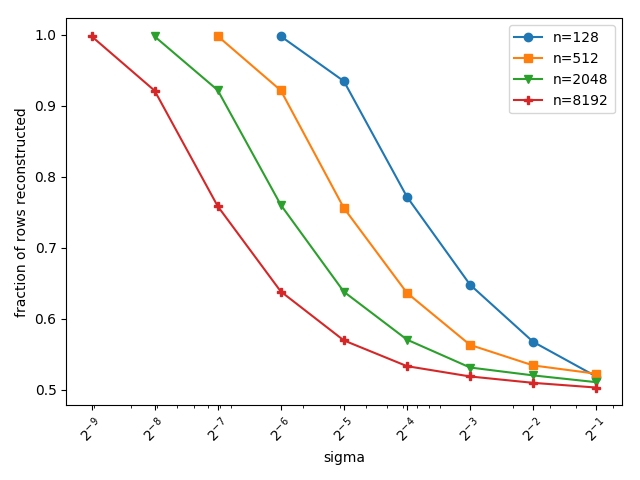
\includegraphics[width=0.5\textwidth]{hadamard_graph.png}
\end{center}

The main takeaway here is that the size of the database $n$ increases, the accuracy value $\alpha=\sigma$ must be much
smaller in order to achieve a complete reconstruction.  Specifically, to achieve the same fraction of reconstruction of
rows for a database four times as large, the error must be twice as small.

For all values of $n$, an error of $\sigma=\frac12$ yielded only a $\frac12$ reconstruction of the dataset, comporable
to random guessing.  For \emph{all} values of $n$, an error of $\sigma=\frac{1}{\sqrt{32n}}$ yielded a near-complete reconstruction
of the entire dataset.

\subsection{Random Query Results}

Unfortunately, all my experiments with $n=8192, m=16n$ failed with a memory error, even on the CS servers.  Any missing
points were attempted, but not completed.

We observed the following results for $n \in \{128, 512, 2048, 8192\}$ and $\sigma \in \{\frac12, \frac14, \frac18,
\ldots, \frac{1}{\sqrt{32n}}\}$.  The vertical lines shown are the standard deviations of the results for each point.
Note the log scale on the lower axis.

\begin{center}
    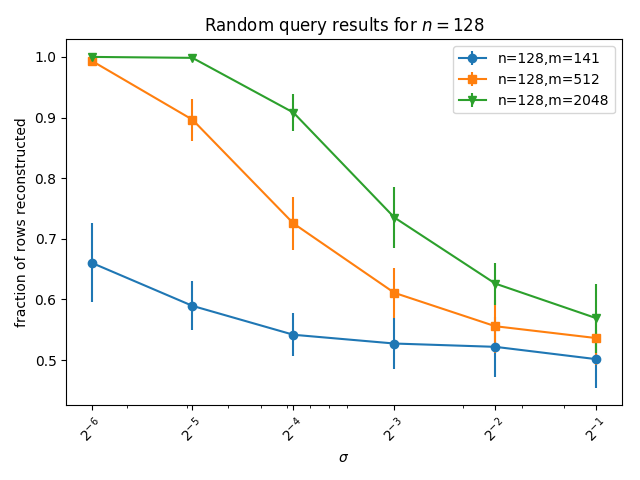
\includegraphics[width=0.49\textwidth]{random_graph_n128.png}
    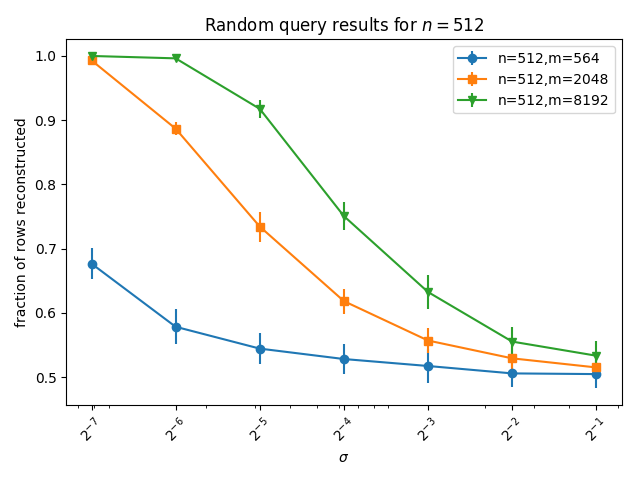
\includegraphics[width=0.49\textwidth]{random_graph_n512.png}

    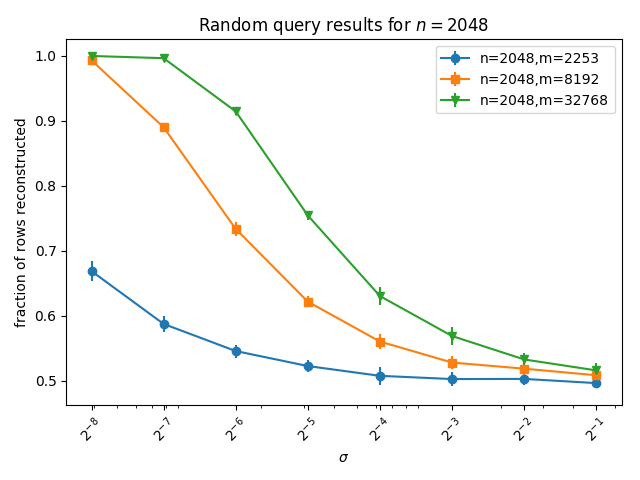
\includegraphics[width=0.49\textwidth]{random_graph_n2048.png}
    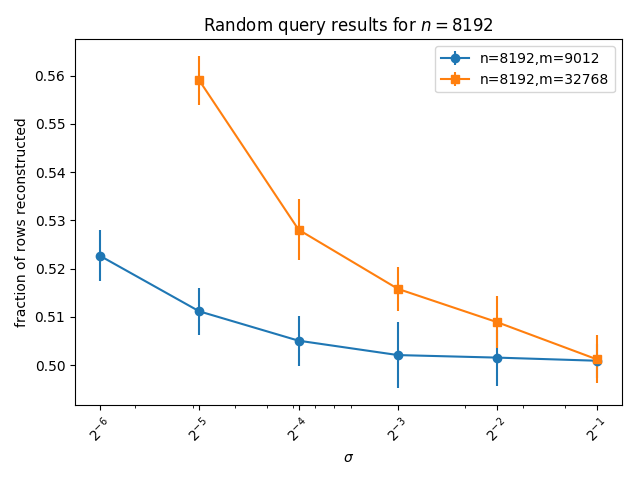
\includegraphics[width=0.49\textwidth]{random_graph_n8192.png}
\end{center}

We see the same dependence on $n$ an $\sigma$ as before, but now we also have a dependence on $m$: For $m=4n, \sigma$
was required to be as low as $2^{-6}$ before the fraction of recovered results approached 1.  As $m$ was increased by
one order of magnitude, one order of magnitude in $\sigma$ was spared.
%\end{document}
